\chapter{Analyses complémentaires des résultats du tests perceptifs}\label{annexe:anova}


\section{Effets des auditeurs sur l'évaluation des scènes}

Pour aller plus loin, une analyse de variance (abrégée ANOVA pour \textit{ANalyse Of VAriance} en anglais) est réalisée afin de déterminer l'influence de chaque auditeur sur l'évaluation des scènes. En effet, selon l'auditeur, l'échelle des notes émises peut varier (un auditeur peut noter sur l'ensemble de l'échelle, d'autres peuvent noter une échelle réduite), influençant l'interprétation des résultats.

C'est ainsi une ANOVA à deux facteurs (\textit{type de scènes} (\textit{enregistré}, \textit{répliqué}) et \textit{auditeur} (50 auditeurs)) avec interaction qui est considérée. De la même manière que le test de Student, l'ANOVA est un outil statistique qui permet de comparer des moyennes d'échantillons et d'étudier l'effet des variables qualitatives (ou facteurs), pouvant prendre plusieurs valeurs (ou niveaux), sur une variable quantitative. Dans ce test, deux hypothèses sont émises sur les distributions :

\begin{itemize}
\item les distributions des échantillons des différentes catégories sont semblables (hypothèse \textit{nulle} $H_0$),
\item les distributions sont différentes, (hypothèse \textit{alternative} $H_1$).\\
\end{itemize}

Pour cela, la statistique de test est la statistique de Fischer $F$. De ces indices, la valeur \textit{p} établit, là encore, la probabilité d'obtenir sous l'hypothèse nulle, des résultats aussi extrêmes que ceux observés. Les résultats sont résumés dans le Tableau \ref{tab:anova_auditeur}. On y résume la somme des carrés des écarts (SCE), les degrés de liberté du système (DDL), la variance, la statistique $F$ et la valeur $p$.

\begin{table}[ht]
\caption{Résultats de l'ANOVA avec interaction avec les facteurs \textit{type} et \textit{auditeur}.}
\centering
\begin{tabular}{lccccc}
\hline
\textbf{Source}     & \textbf{SCE} & \textbf{DDL} & \textbf{variance} & \textbf{F} & \textbf{p-valeur} \\
\hline
\textbf{auditeur} & 687,93 & 49 & 14,03 & 7,89 & <1e-4 \\
\hline
\textbf{type} & 3,61 & 1 & 3,61 & 1,82 & 0,18 \\
\hline
\textbf{auditeur$*$type} & 93,29 & 49 & 0,90 & 0,55 & 0,55 \\
\hline
\textbf{erreur}      & 1780,42 & 899 & 1,98 & &  \\
\hline
\textbf{total}      & 2572 & 998 & & & \\
\hline
\end{tabular}
\label{tab:anova_auditeur}
\end{table}

Le facteur \textit{auditeur} a une influence significative (valeur $p$ < $\alpha$) révélant que les auditeurs n'ont pas les mêmes échelles d'évaluation. L'influence du facteur \textit{type} reste toujours non significative. Son interaction avec le facteur \textit{auditeur} est non-significatif également.
Le phénomène d'interaction traduit l'influence des différents niveaux d'un facteur sur l'autre facteur. Ici, l'interaction entre le facteur \textit{auditeur} et \textit{type} est non-significative, ce qui signifie que pour chaque juge, la perception des scènes est similaire, même si entre chaque juge des dissimilarités existent.

\section{Effets de l'ambiance sonore}

Une seconde ANOVA à deux facteurs avec interaction est effectuée avec pour facteur le \textit{type} (\textit{enregistrée}, \textit{répliquée}) et l'\textit{ambiance sonore} (\textit{parc, rue calme, rue bruyante, rue très bruyante}) afin de déterminer si la perception du réalisme est différent selon l'ambiance sonore. Les résultats de l'ANOVA sont résumés dans le Tableau \ref{tab:anova_ambiance}.

\begin{table}[ht]
\caption{Résultats de l'ANOVA avec interaction avec les facteurs \textit{type} et \textit{ambiance}.}
\centering
\begin{tabular}{lccccc}
\hline
\textbf{Source}     & \textbf{SCE} & \textbf{DDL} & \textbf{variance} & \textbf{F} & \textbf{p-valeur} \\
\hline
\textbf{type} & 5,72 & 1 & 5,72 & 2,28 & 0,13 \\
\hline
\textbf{ambiance} & 42,65 & 3 & 14,21 & 5,66 & 8,00e-4 \\
\hline
\textbf{type/ambiance} & 36,83 & 3 & 12,27 & 4,89 & 2,20e-3 \\
\hline
\textbf{erreur}      & 2488,49 & 991 & 2,55 & &  \\
\hline
\textbf{total}      & 2572 & 998 & & & \\
\hline
\end{tabular}
\label{tab:anova_ambiance}
\end{table}


Si l'impact du facteur \textit{type} est toujours non significatif, celui du facteur \textit{ambiance} et l'interaction entre les deux facteurs sont toutefois significatifs ($p < \alpha$). L'influence principale du facteur \textit{ambiance} signifie qu'il y a une distinction entre les distributions des notes selon l'ambiance sonore. Le phénomène d'interaction traduit le fait que l'effet du type de scène (enregistré - répliqué) sur le réalisme varie en fonction de l'ambiance considérée.

Pour visualiser ce phénomène d'interaction entre le type de scènes et l'ambiance sonore, l'évolution de la note moyenne dans chaque cas est tracée (Figure \ref{fig:interaction_ambianceType}). On observe que selon l'ambiance sonore, la note de réalisme des scènes répliquées peut être inférieure ou supérieure par rapport aux scènes enregistrées. Cette évolution traduit une interaction croisée dont l'origine est toutefois difficile à estimer. 

\begin{figure}[h]
\centering
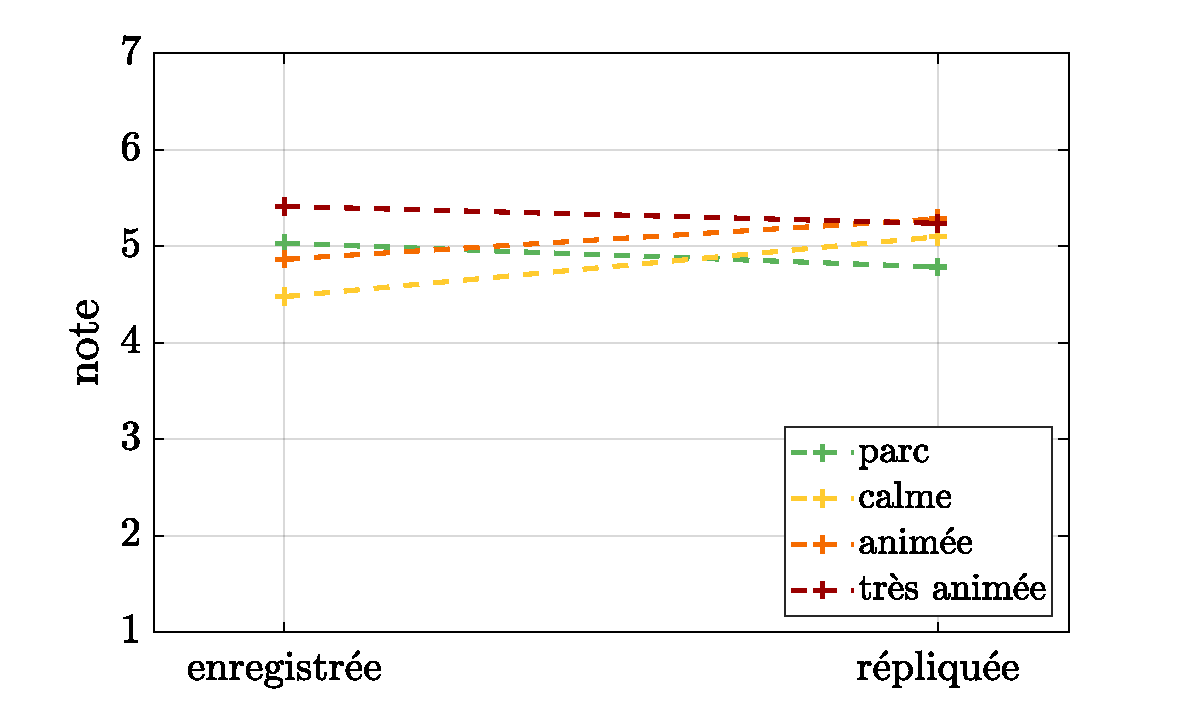
\includegraphics[width=0.8\linewidth]{./figures/test_perceptif/testPerceptif_interactionAmbiance.pdf}
\caption{Diagramme des effets d'intéraction type$*$ambiance.}\label{fig:interaction_ambianceType}
\end{figure}


Même si les moyennes globales et les distributions entre les scènes enregistrées et répliquées sont similaires, des disparités existent selon les auditeurs ou les ambiances sonores sans toutefois que celles-ci remettent en cause les similarités entre les deux types.\\